\documentclass[14pt,a4paper]{extarticle}
% =============================================================
% preamble.tex — оформление отчётов по СТП БГУИР 01-2024
% =============================================================

% Шрифты: под pdflatex — Times через tempora + T2A,
% под xelatex/tectonic — системный Times New Roman (запасной вариант STIX Two Text)
\usepackage{iftex}
\ifPDFTeX
  \usepackage[utf8]{inputenc}
  \usepackage[T2A]{fontenc}
  \usepackage{tempora}
\else
  \usepackage{fontspec}
  \IfFontExistsTF{Times New Roman}
    {\setmainfont{Times New Roman}}
    {\setmainfont{STIX Two Text}}
  \IfFontExistsTF{DejaVu Sans Mono}
    {\setmonofont{DejaVu Sans Mono}[Scale=0.82]}
    {\setmonofont{DejaVuSansMono}[Extension=.ttf, BoldFont=*-Bold,
                                  ItalicFont=*-Oblique, Scale=0.82]}
\fi
\usepackage[russian]{babel}

% Поля: слева 30 мм, справа 15 мм, сверху и снизу 20 мм
\usepackage{geometry}
\geometry{left=30mm, right=15mm, top=20mm, bottom=20mm}

\usepackage{setspace}
\singlespacing

\pretolerance=1000
\tolerance=2000
\emergencystretch=3em

\usepackage{indentfirst}
\setlength{\parindent}{1.25cm}

% Номер страницы — снизу справа
\usepackage{fancyhdr}
\pagestyle{fancy}
\fancyhf{}
\fancyfoot[R]{\thepage}
\renewcommand{\headrulewidth}{0pt}
\fancypagestyle{plain}{%
  \fancyhf{}%
  \fancyfoot[R]{\thepage}%
  \renewcommand{\headrulewidth}{0pt}%
}

\usepackage{amsmath,amssymb}
\usepackage{graphicx}
\usepackage{float}
\usepackage{booktabs}
\usepackage{tabularx}
\usepackage{multirow}
\usepackage{longtable}
\usepackage{array}

\usepackage{caption}
\captionsetup[figure]{labelsep=endash, justification=centering,
                      font={normalsize}, name=Рисунок}
\captionsetup[table]{labelsep=endash, justification=raggedright,
                     singlelinecheck=false, font={normalsize}, name=Таблица}

\usepackage{titlesec}
\titleformat{\section}
  {\normalfont\fontsize{14}{18}\selectfont\bfseries}
  {\thesection}{0.5em}{\MakeUppercase}
\titlespacing*{\section}{1.25cm}{0pt}{14pt}
% Разрыв страницы до заголовка, чтобы номер в содержании совпадал со страницей раздела
\newcommand{\sectionbreak}{\clearpage}
\titleformat{\subsection}
  {\normalfont\fontsize{14}{18}\selectfont\bfseries}
  {\thesubsection}{0.5em}{}
\titlespacing*{\subsection}{1.25cm}{14pt}{14pt}
\titleformat{\subsubsection}
  {\normalfont\fontsize{14}{18}\selectfont\bfseries}
  {\thesubsubsection}{0.5em}{}
\titlespacing*{\subsubsection}{1.25cm}{14pt}{14pt}

\newcommand{\sectioncenter}[1]{%
  \newpage
  \phantomsection
  \addcontentsline{toc}{section}{#1}
  \begin{center}\textbf{\MakeUppercase{#1}}\end{center}
  \vspace{14pt}
}

\usepackage{tocloft}
\renewcommand{\cftsecfont}{\normalfont}
\renewcommand{\cftsecpagefont}{\normalfont}
\renewcommand{\cftsubsecfont}{\normalfont}
\renewcommand{\cftsubsecpagefont}{\normalfont}
\renewcommand{\cftsecleader}{\cftdotfill{\cftdotsep}}
\renewcommand{\cftdotsep}{1}
% babel переопределяет заголовки после преамбулы, поэтому правим через \addto
\addto\captionsrussian{\renewcommand{\contentsname}{\hfill\textbf{СОДЕРЖАНИЕ}\hfill}}
\renewcommand{\cftaftertoctitle}{\hfill}

\usepackage{enumitem}
\setlist[itemize]{noitemsep, topsep=0pt, leftmargin=1.25cm, label=--}
\setlist[enumerate]{noitemsep, topsep=0pt, leftmargin=1.25cm}

% Листинги кода и вывода программы
\usepackage{listings}
\usepackage{fancyvrb}
\lstset{
  basicstyle=\ttfamily\footnotesize,
  frame=single,
  breaklines=true,
  showstringspaces=false,
  inputencoding=utf8,
  extendedchars=true,
  columns=fullflexible,
  keepspaces=true,
  captionpos=t
}
\ifPDFTeX
\lstset{
  literate={а}{{\cyra}}1 {б}{{\cyrb}}1 {в}{{\cyrv}}1 {г}{{\cyrg}}1
           {д}{{\cyrd}}1 {е}{{\cyre}}1 {ж}{{\cyrzh}}1 {з}{{\cyrz}}1
           {и}{{\cyri}}1 {й}{{\cyrishrt}}1 {к}{{\cyrk}}1 {л}{{\cyrl}}1
           {м}{{\cyrm}}1 {н}{{\cyrn}}1 {о}{{\cyro}}1 {п}{{\cyrp}}1
           {р}{{\cyrr}}1 {с}{{\cyrs}}1 {т}{{\cyrt}}1 {у}{{\cyru}}1
           {ф}{{\cyrf}}1 {х}{{\cyrh}}1 {ц}{{\cyrc}}1 {ч}{{\cyrch}}1
           {ш}{{\cyrsh}}1 {щ}{{\cyrshch}}1 {ъ}{{\cyrhrdsn}}1
           {ы}{{\cyrery}}1 {ь}{{\cyrsftsn}}1 {э}{{\cyrerev}}1
           {ю}{{\cyryu}}1 {я}{{\cyrya}}1 {ё}{{\cyryo}}1
           {А}{{\CYRA}}1 {Б}{{\CYRB}}1 {В}{{\CYRV}}1 {Г}{{\CYRG}}1
           {Д}{{\CYRD}}1 {Е}{{\CYRE}}1 {Ж}{{\CYRZH}}1 {З}{{\CYRZ}}1
           {И}{{\CYRI}}1 {Й}{{\CYRISHRT}}1 {К}{{\CYRK}}1 {Л}{{\CYRL}}1
           {М}{{\CYRM}}1 {Н}{{\CYRN}}1 {О}{{\CYRO}}1 {П}{{\CYRP}}1
           {Р}{{\CYRR}}1 {С}{{\CYRS}}1 {Т}{{\CYRT}}1 {У}{{\CYRU}}1
           {Ф}{{\CYRF}}1 {Х}{{\CYRH}}1 {Ц}{{\CYRC}}1 {Ч}{{\CYRCH}}1
           {Ш}{{\CYRSH}}1 {Щ}{{\CYRSHCH}}1 {Ъ}{{\CYRHRDSN}}1
           {Ы}{{\CYRERY}}1 {Ь}{{\CYRSFTSN}}1 {Э}{{\CYREREV}}1
           {Ю}{{\CYRYU}}1 {Я}{{\CYRYA}}1 {Ё}{{\CYRYO}}1
           {—}{{---}}1 {–}{{--}}1 {…}{{\ldots}}1
}
\fi

% Подписи листингов — в том же стиле, что таблицы: «Листинг X.Y — Название»
\captionsetup[lstlisting]{labelsep=endash, justification=raggedright,
                          singlelinecheck=false, font={normalsize}}
\renewcommand{\lstlistingname}{Листинг}
\AtBeginDocument{\numberwithin{lstlisting}{section}}

\lstdefinestyle{python}{language=Python, keywordstyle=\bfseries}
\lstdefinestyle{shell}{language=bash, keywordstyle=\mdseries}
\lstdefinestyle{plain}{language={}, basicstyle=\ttfamily\scriptsize}

% Абзац после листинга должен сохранять отступ 1,25 см (СТП 2.1.1)
\makeatletter
\AtBeginDocument{\let\@endpetrue\@endpefalse}
\makeatother

% Подпись к блоку verbatim: \captionof вне плавающего окружения
% глобально обнуляет \parindent, поэтому отступ восстанавливается вручную
\newcommand{\listingcaption}[2]{%
  \captionof{lstlisting}{#1}\label{#2}%
  \setlength{\parindent}{1.25cm}%
}

\usepackage{hyperref}
\hypersetup{colorlinks=true, linkcolor=black, urlcolor=blue, citecolor=black}

\numberwithin{figure}{section}
\numberwithin{table}{section}
\numberwithin{equation}{section}

% Титульный лист отчёта по лабораторной работе
\newcommand{\makelabtitle}[2]{%
  \begin{titlepage}
  \thispagestyle{empty}
  \begin{center}

  МИНИСТЕРСТВО ОБРАЗОВАНИЯ РЕСПУБЛИКИ БЕЛАРУСЬ

  \vspace{0.5em}
  Учреждение образования

  \vspace{0.5em}
  \textbf{<<Белорусский государственный университет информатики и радиоэлектроники>>}

  \vspace{2em}
  Факультет компьютерных систем и сетей

  \vspace{0.5em}
  Кафедра программного обеспечения информационных технологий
  \end{center}

  \vspace{3em}
  \begin{center}
  \textbf{ОТЧЕТ}

  \vspace{0.5em}
  по лабораторной работе №#1

  \vspace{0.5em}
  по дисциплине

  \vspace{0.5em}
  <<Технологии компонентного программирования>>

  \vspace{0.5em}
  <<#2>>
  \end{center}

  \vspace{5em}
  \begin{flushright}
  \begin{minipage}{0.5\textwidth}
  \textbf{Выполнил:}\\
  Лебедевич Артем Владимирович\\
  магистрант группы 556301

  \vspace{0.6em}
  \textbf{Преподаватель:}\\
  Герман Олег Витольдович\\
  кандидат технических наук\\
  доцент кафедры ИТАС
  \end{minipage}
  \end{flushright}

  \vfill
  \begin{center}Минск, 2026~г.\end{center}
  \end{titlepage}
}


\newcolumntype{L}{>{\raggedright\arraybackslash}X}
\lstdefinestyle{java}{language=Java, keywordstyle=\bfseries}
\lstdefinestyle{jsp}{language=HTML, basicstyle=\ttfamily\scriptsize, keywordstyle=\mdseries}

\begin{document}

\makelabtitle{5}{JSP: активные страницы Java на сервере Tomcat}

\tableofcontents

\section{Цель работы}

Изучить технологию JSP (Java Server Pages) и компоненты JavaBeans на web-сервере
Apache Tomcat. Используя приложение из методических материалов как прототип, создать
JSP-приложения: выдачу курсов доллара и евро по названию валюты, страницу, которая
возвращает изображение, переводчик слов с английского на русский и обратно из
ограниченного лексикона и программу, передающую клиенту сайт через объект
\texttt{PrintWriter}.

\section{Теоретические сведения}

\subsection{JSP и Tomcat}

JSP-страница --- это HTML-документ со вставками кода на Java. Страницы не нужно
компилировать вручную: при первом обращении сервер Tomcat (компонент Jasper)
преобразует страницу в исходный текст сервлета, компилирует его встроенным
компилятором Eclipse (ecj) и далее для каждого запроса вызывает метод
\texttt{\_jspService}. Основные элементы страницы приведены в
таблице~\ref{tab:terms}.

\begin{table}[H]
\caption{Элементы JSP}
\label{tab:terms}
\centering
\begin{tabularx}{\textwidth}{>{\raggedright\arraybackslash}p{0.42\textwidth}L}
\toprule
Элемент & Смысл \\
\midrule
\texttt{<\%-{}- -{}-\%>} & комментарий \\
\texttt{<\%@ page import="..." \%>} & директива: импорт классов, тип содержимого,
кодировка \\
\texttt{<\%@ include file="..." \%>} & директива: вставка текста другого файла до
компиляции \\
\texttt{<\%! ... \%>} & объявление поля или метода класса сервлета \\
\texttt{<\% ... \%>} & скриптлет: код внутри \texttt{\_jspService} \\
\texttt{<\%= ... \%>} & выражение: значение выводится в страницу \\
\texttt{request}, \texttt{response}, \texttt{out}, \texttt{session} & неявные
объекты, доступные на каждой странице \\
\texttt{jsp:useBean}, \texttt{jsp:\allowbreak setProperty}, \texttt{jsp:\allowbreak getProperty} & создание
компонента в области видимости, заполнение свойства из параметра запроса, вывод
свойства \\
\bottomrule
\end{tabularx}
\end{table}

Компонент JavaBean --- класс с открытым конструктором без параметров и свойствами,
доступными через методы \texttt{getX} и \texttt{setX}. Действие
\texttt{<jsp:setProperty property="name">} вызывает \texttt{setName} со значением
параметра запроса \texttt{name}, поэтому поле формы и свойство компонента связываются
по имени. Область \texttt{session} сохраняет компонент между запросами одного
пользователя.

Web-приложение размещается на сервере в виде архива WAR: в корне лежат страницы, в
каталоге \texttt{WEB-INF} --- дескриптор \texttt{web.xml} и откомпилированные классы.
Архив создаётся утилитой \texttt{jar} и копируется в каталог \texttt{webapps}.

\subsection{Различия при работе с JDK 17}

Методичка рассчитана на Tomcat 8.5.5 и Java 8. С JDK 17 обнаружились следующие
отличия.

\begin{itemize}
\item Tomcat 8.5.5 из методических материалов запускается, однако его компилятор
ecj 4.5.1 не читает часть классов JDK 17: страница, обращающаяся к
\texttt{System}, завершается ошибкой \texttt{ClassFormatException: Failed to load
class [java.lang.System]}. Последняя версия ветки 8.5 (8.5.100, ecj 4.6.3) ведёт себя
так же. Использован Tomcat 9.0.122: он сохраняет API \texttt{javax.servlet} методички и
содержит ecj 4.20.
\item В примере \texttt{ImageServlet.jsp} поток назван \texttt{OutputStream out}, но имя
\texttt{out} уже занято неявным объектом \texttt{JspWriter}, и страница не
компилируется. Поток назван \texttt{os}, а атрибут
\texttt{trimDirectiveWhitespaces="true"} не допускает в двоичный ответ переводы строк
между директивами.
\item Вместо среды NetBeans архив собирается командами \texttt{javac} и \texttt{jar},
как в лекции по Tomcat.
\end{itemize}

\section{Реализация}

\subsection{Структура программы}

\listingcaption{Структура лабораторной работы}{lst:tree}
\begin{Verbatim}[fontsize=\scriptsize, frame=single, samepage=true]
lab5/java/com/Hello.java         компонент прототипа (свойство name)
lab5/java/com/CurrencyBean.java  курс доллара и евро (НБ РБ или таблица)
lab5/java/com/Dictionary.java    англо-русский словарь из 38 пар слов
lab5/webapp/index.jsp            Hello from JSP, TODAY IS, оглавление
lab5/webapp/hello.jsp, response.jsp   прототип: форма и компонент сессии
lab5/webapp/currency.jsp, rate.jsp    задание 1: курсы валют
lab5/webapp/image.html, ImageServlet.jsp  задание 2: изображение PNG
lab5/webapp/translate.jsp        задание 3: переводчик
lab5/webapp/site.jsp             задание 4: сайт через PrintWriter
lab5/webapp/header.jspf, style.css, WEB-INF/web.xml
lab5/runtime.py                  сборка lab5.war, запуск Tomcat
lab5/cases.py                    проверяемые сценарии по HTTP
lab5/runner.py, gui.py, server.py  консоль, окно, сервер
\end{Verbatim}

\subsection{Сборка и запуск}

Модуль \texttt{lab5/runtime.py} компилирует компоненты
(\texttt{javac -{}-release 8}) в каталог \texttt{WEB-INF/classes}, упаковывает
приложение командой \texttt{jar -cf lab5.war} и создаёт отдельный каталог
\texttt{CATALINA\_BASE} с собственным \texttt{server.xml} (порт 8040). Установленный
Tomcat при этом не изменяется. Сервер запускается классом
\texttt{org.apache.catalina.startup.Bootstrap}; приложение доступно по адресу
\texttt{http://127.0.0.1:8040/lab5/}. Скрипт \texttt{scripts/fetch\_runtimes.py}
скачивает Tomcat и проверяет контрольную сумму SHA-512.

\subsection{Прототип}

Страница \texttt{index.jsp} повторяет пример методички: метод \texttt{getDate} объявлен
тегом \texttt{<\%!} и выводится выражением \texttt{<\%=}. Форма \texttt{hello.jsp}
передаёт имя странице \texttt{response.jsp}, которая заполняет компонент
\texttt{com.Hello} в области \texttt{session} и выводит приветствие.

\subsection{Задание 1: курсы валют}

По образцу прототипа форма \texttt{currency.jsp} передаёт название валюты странице
\texttt{rate.jsp} (листинг~\ref{lst:rate}). Компонент \texttt{CurrencyBean} понимает
названия \texttt{dollar}, \texttt{USD}, \texttt{\$}, \texttt{доллар}, \texttt{euro},
\texttt{EUR}, \texttt{евро} в любом регистре. Курс запрашивается у Национального банка
Республики Беларусь (\texttt{api.nbrb.by}) один раз в день; без доступа к сети
используется встроенная таблица, и страница указывает источник.

\begin{lstlisting}[style=jsp, caption={Страница rate.jsp}, label={lst:rate}]
<jsp:useBean id="currency" scope="session" class="com.CurrencyBean" />
<jsp:setProperty name="currency" property="name" />
<% if (currency.getName() == null) { %>
<p class="error">No currency entered yet.</p>
<% } else if (!currency.isKnown()) { %>
<p class="error">Unknown currency ... Only the dollar and the euro are supported.</p>
<% } else { %>
<p class="answer">1 <jsp:getProperty name="currency" property="code" /> =
  <jsp:getProperty name="currency" property="rate" /> BYN</p>
<p>Date <jsp:getProperty name="currency" property="date" />,
  source: <jsp:getProperty name="currency" property="source" /></p>
<% } %>
\end{lstlisting}

\begin{lstlisting}[style=java, caption={Свойство name компонента CurrencyBean}, label={lst:bean}]
public void setName(String name) {
    this.name = name;
    this.code = name == null ? null : ALIASES.get(name.trim().toLowerCase(Locale.ROOT));
    if (code != null) {
        load();  // NBRB once a day, the built-in table without the network
    }
}

public String getRate() {
    return code == null ? "" : String.format(Locale.ROOT, "%.4f", rate);
}
\end{lstlisting}

\subsection{Задание 2: изображение}

Страница \texttt{ImageServlet.jsp} объявляет тип содержимого \texttt{image/png},
рисует в \texttt{BufferedImage} средствами \texttt{Graphics2D} фон, синусоиду, солнце и
текст из параметра запроса и записывает картинку методом \texttt{ImageIO.write} в
двоичный поток ответа (листинг~\ref{lst:image}). Страница \texttt{image.html} выводит
её тегом \texttt{<img src="ImageServlet.jsp">}; форма на странице меняет текст и
перерисовывает изображение.

\begin{lstlisting}[style=java, caption={Страница ImageServlet.jsp (фрагмент)}, label={lst:image}]
BufferedImage bufferedImage = new BufferedImage(width, height, BufferedImage.TYPE_INT_RGB);
Graphics2D g2d = bufferedImage.createGraphics();
g2d.setColor(Color.BLUE);
g2d.fillRect(0, 0, width, height);
// ... sine wave, sun
g2d.setColor(Color.WHITE);
g2d.setFont(new Font("SansSerif", Font.BOLD, Math.max(12, height / 8)));
g2d.drawString(text, width / 10, height / 2);
g2d.dispose();

response.setContentType("image/png");
OutputStream os = response.getOutputStream();  // "out" is the implicit JspWriter
ImageIO.write(bufferedImage, "png", os);
os.close();
\end{lstlisting}

\subsection{Задание 3: переводчик}

Компонент \texttt{com.Dictionary} хранит 38 пар слов. Направление перевода
определяется по алфавиту: если в слове есть кириллица, слово переводится с русского на
английский, иначе --- с английского на русский. Регистр и лишние пробелы не
учитываются. Страница \texttt{translate.jsp} использует компонент в области
\texttt{request}, выводит перевод или сообщение о том, что слова нет в лексиконе, и
показывает весь лексикон ссылками.

\subsection{Задание 4: сайт через PrintWriter}

В примере методички объект \texttt{ot = response.getWriter()} возвращает клиенту строку
\texttt{TODAY IS}. Страница \texttt{site.jsp} не содержит HTML-шаблона: метод
\texttt{writeSite} (листинг~\ref{lst:site}) выводит через \texttt{ot} весь сайт ---
заголовок, стили, меню из четырёх страниц, выбранную страницу и подвал. Страница
выбирается параметром \texttt{page}; неизвестное значение заменяется главной страницей.

\begin{lstlisting}[style=java, caption={Вывод сайта через PrintWriter}, label={lst:site}]
void writeSite(PrintWriter ot, String page, String server) {
    ot.println("<!DOCTYPE html>");
    ot.println("<html lang=\"en\"><head><meta charset=\"UTF-8\">");
    ...
    ot.print("<nav>");
    for (String[] item : PAGES) {
        String on = item[0].equals(page) ? " class=\"on\"" : "";
        ot.print("<a" + on + " href=\"site.jsp?page=" + item[0] + "\">" + item[1] + "</a>");
    }
    ot.println("</nav>");
    ...
}
<%
    PrintWriter ot = response.getWriter();
    writeSite(ot, known ? page_ : "home", application.getServerInfo());
%>
\end{lstlisting}

\subsection{Окно проверки}

Окно \texttt{python main.py -{}-lab 5 -{}-gui} написано на wxPython: кнопки открывают
страницы приложения во встроенном браузере, справа расположен список из восьми
сценариев. Команда \texttt{python -m lab5.server} оставляет Tomcat запущенным для
работы в обычном браузере.

\section{Результаты работы программы}

На рисунке~\ref{fig:window} показано окно после выполнения всех сценариев (8 из 8) с
главной страницей приложения.

\begin{figure}[H]
\centering
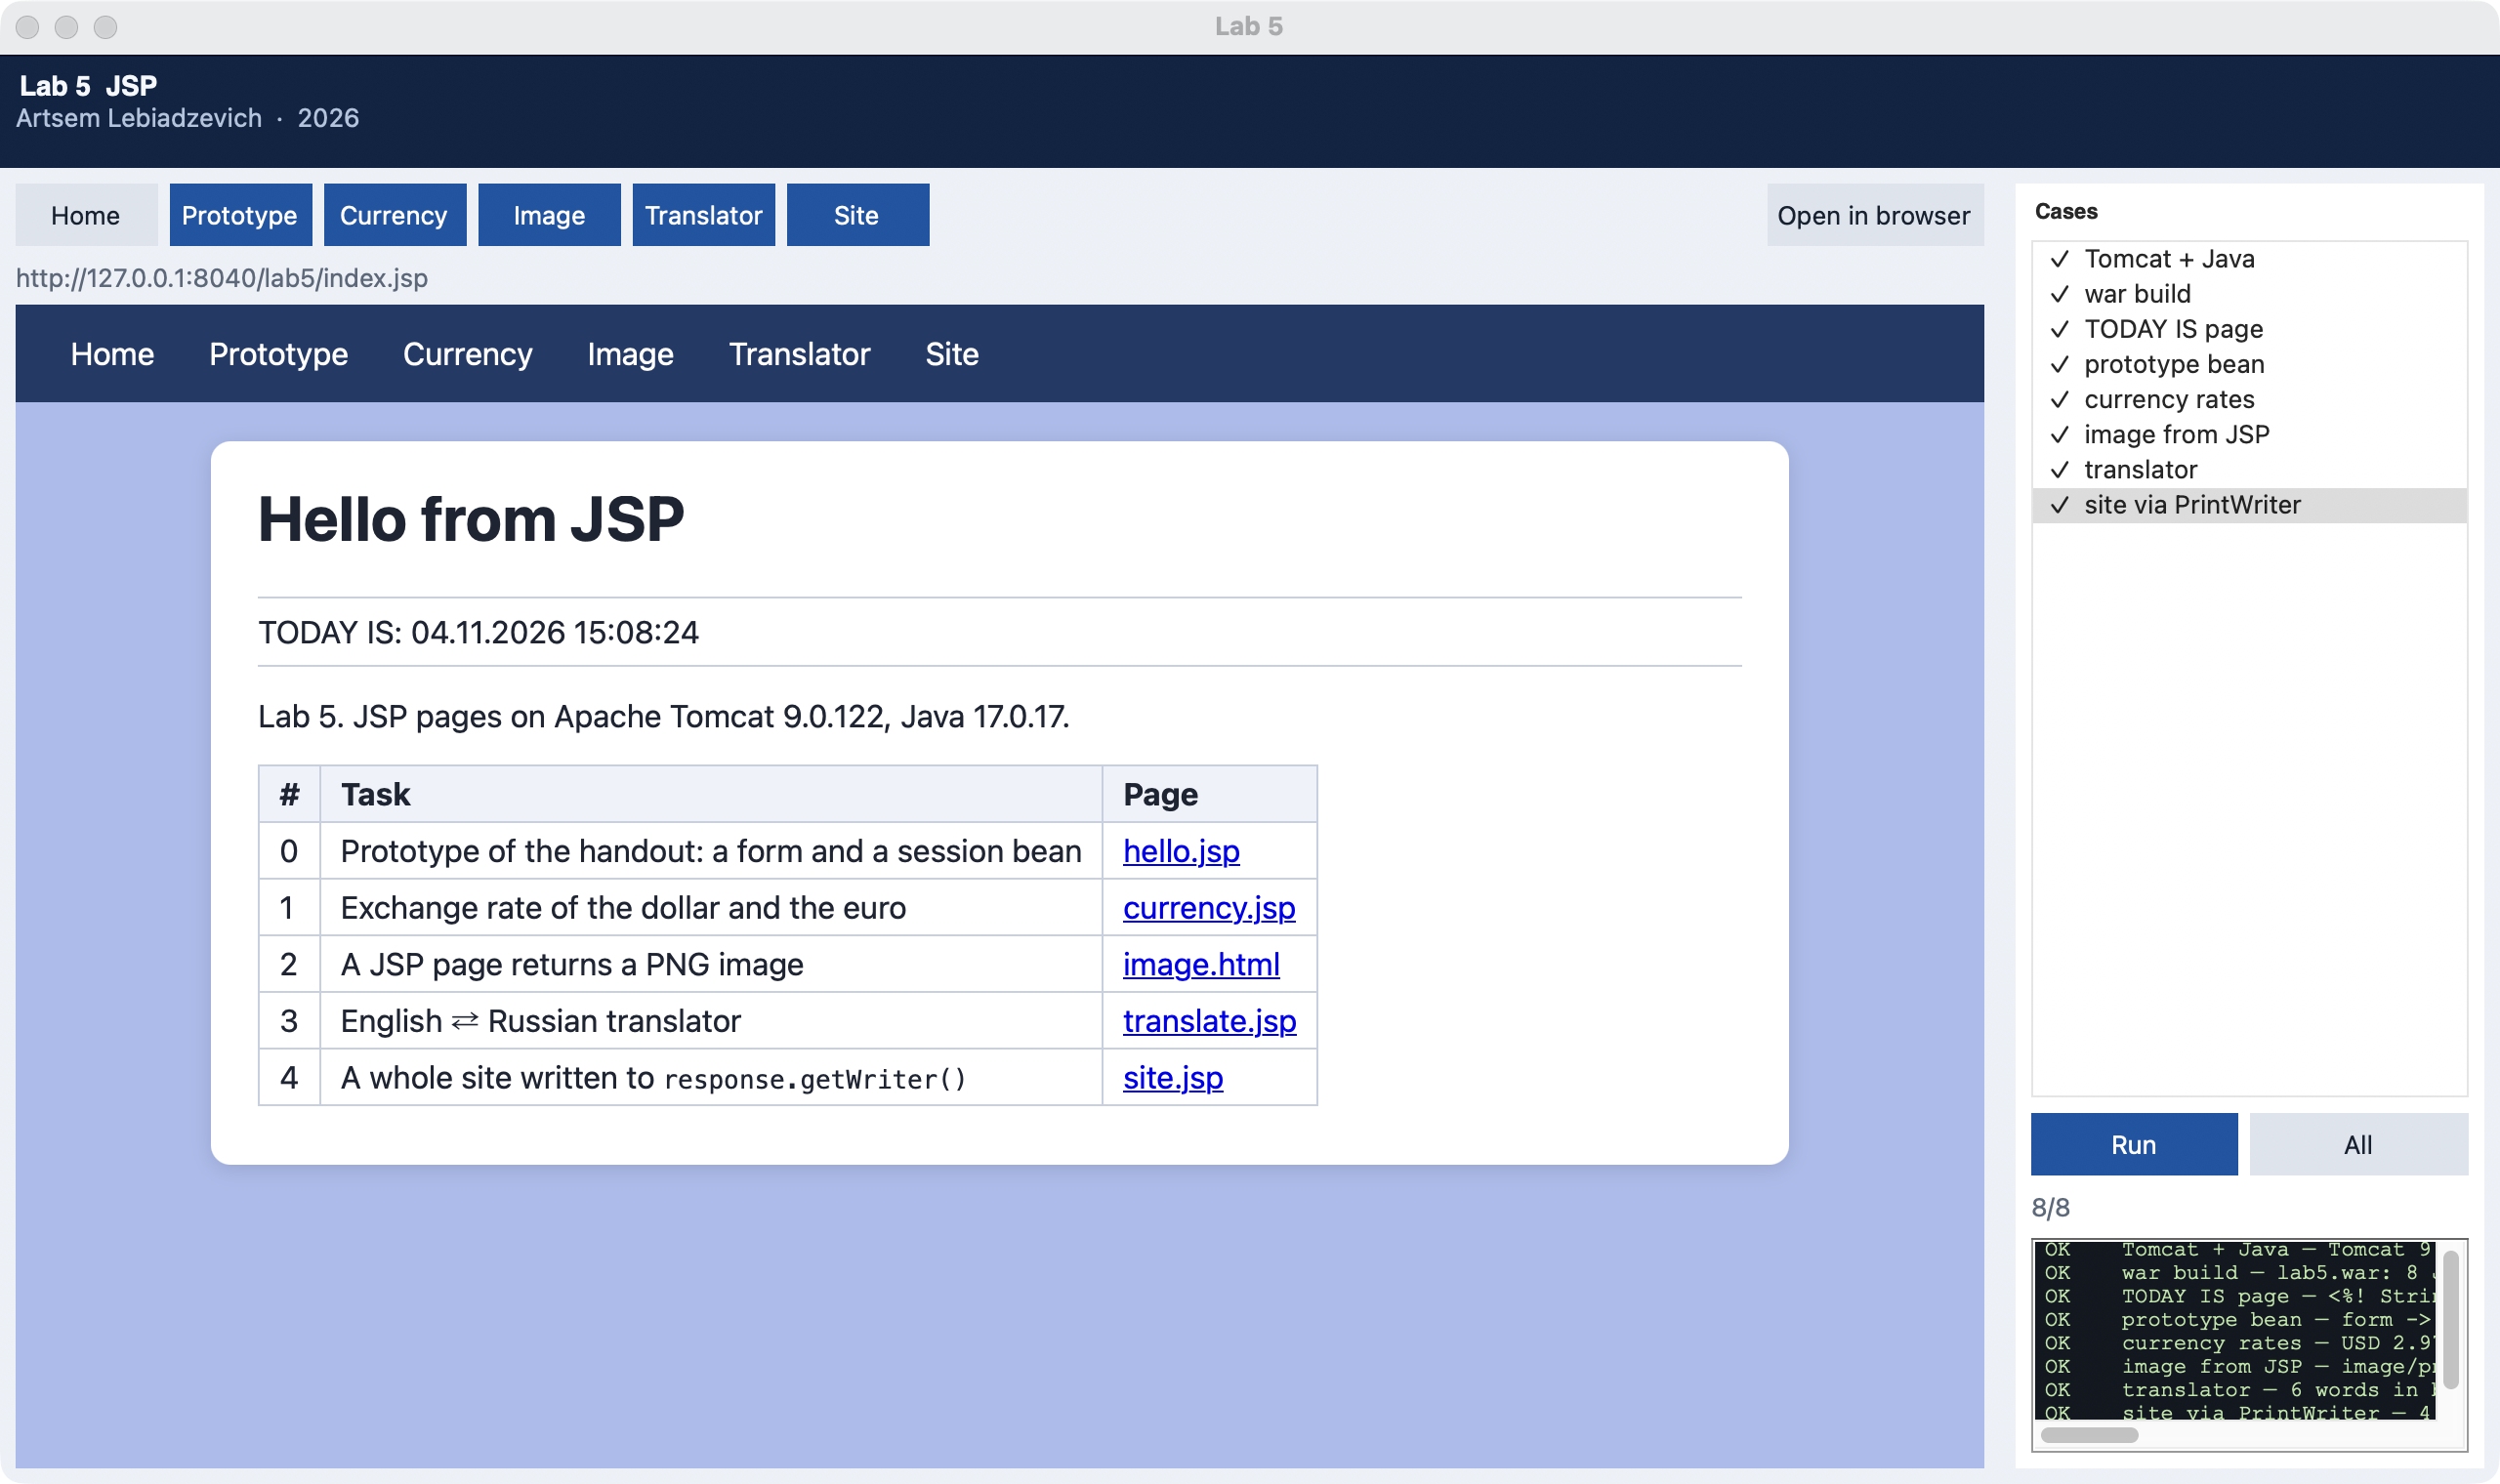
\includegraphics[width=0.95\textwidth]{../screenshots/lab5.png}
\caption{Окно лабораторной работы: главная страница и список проверок}
\label{fig:window}
\end{figure}

Результаты четырёх заданий показаны на рисунках~\ref{fig:currency}--\ref{fig:site}.

\begin{figure}[H]
\centering
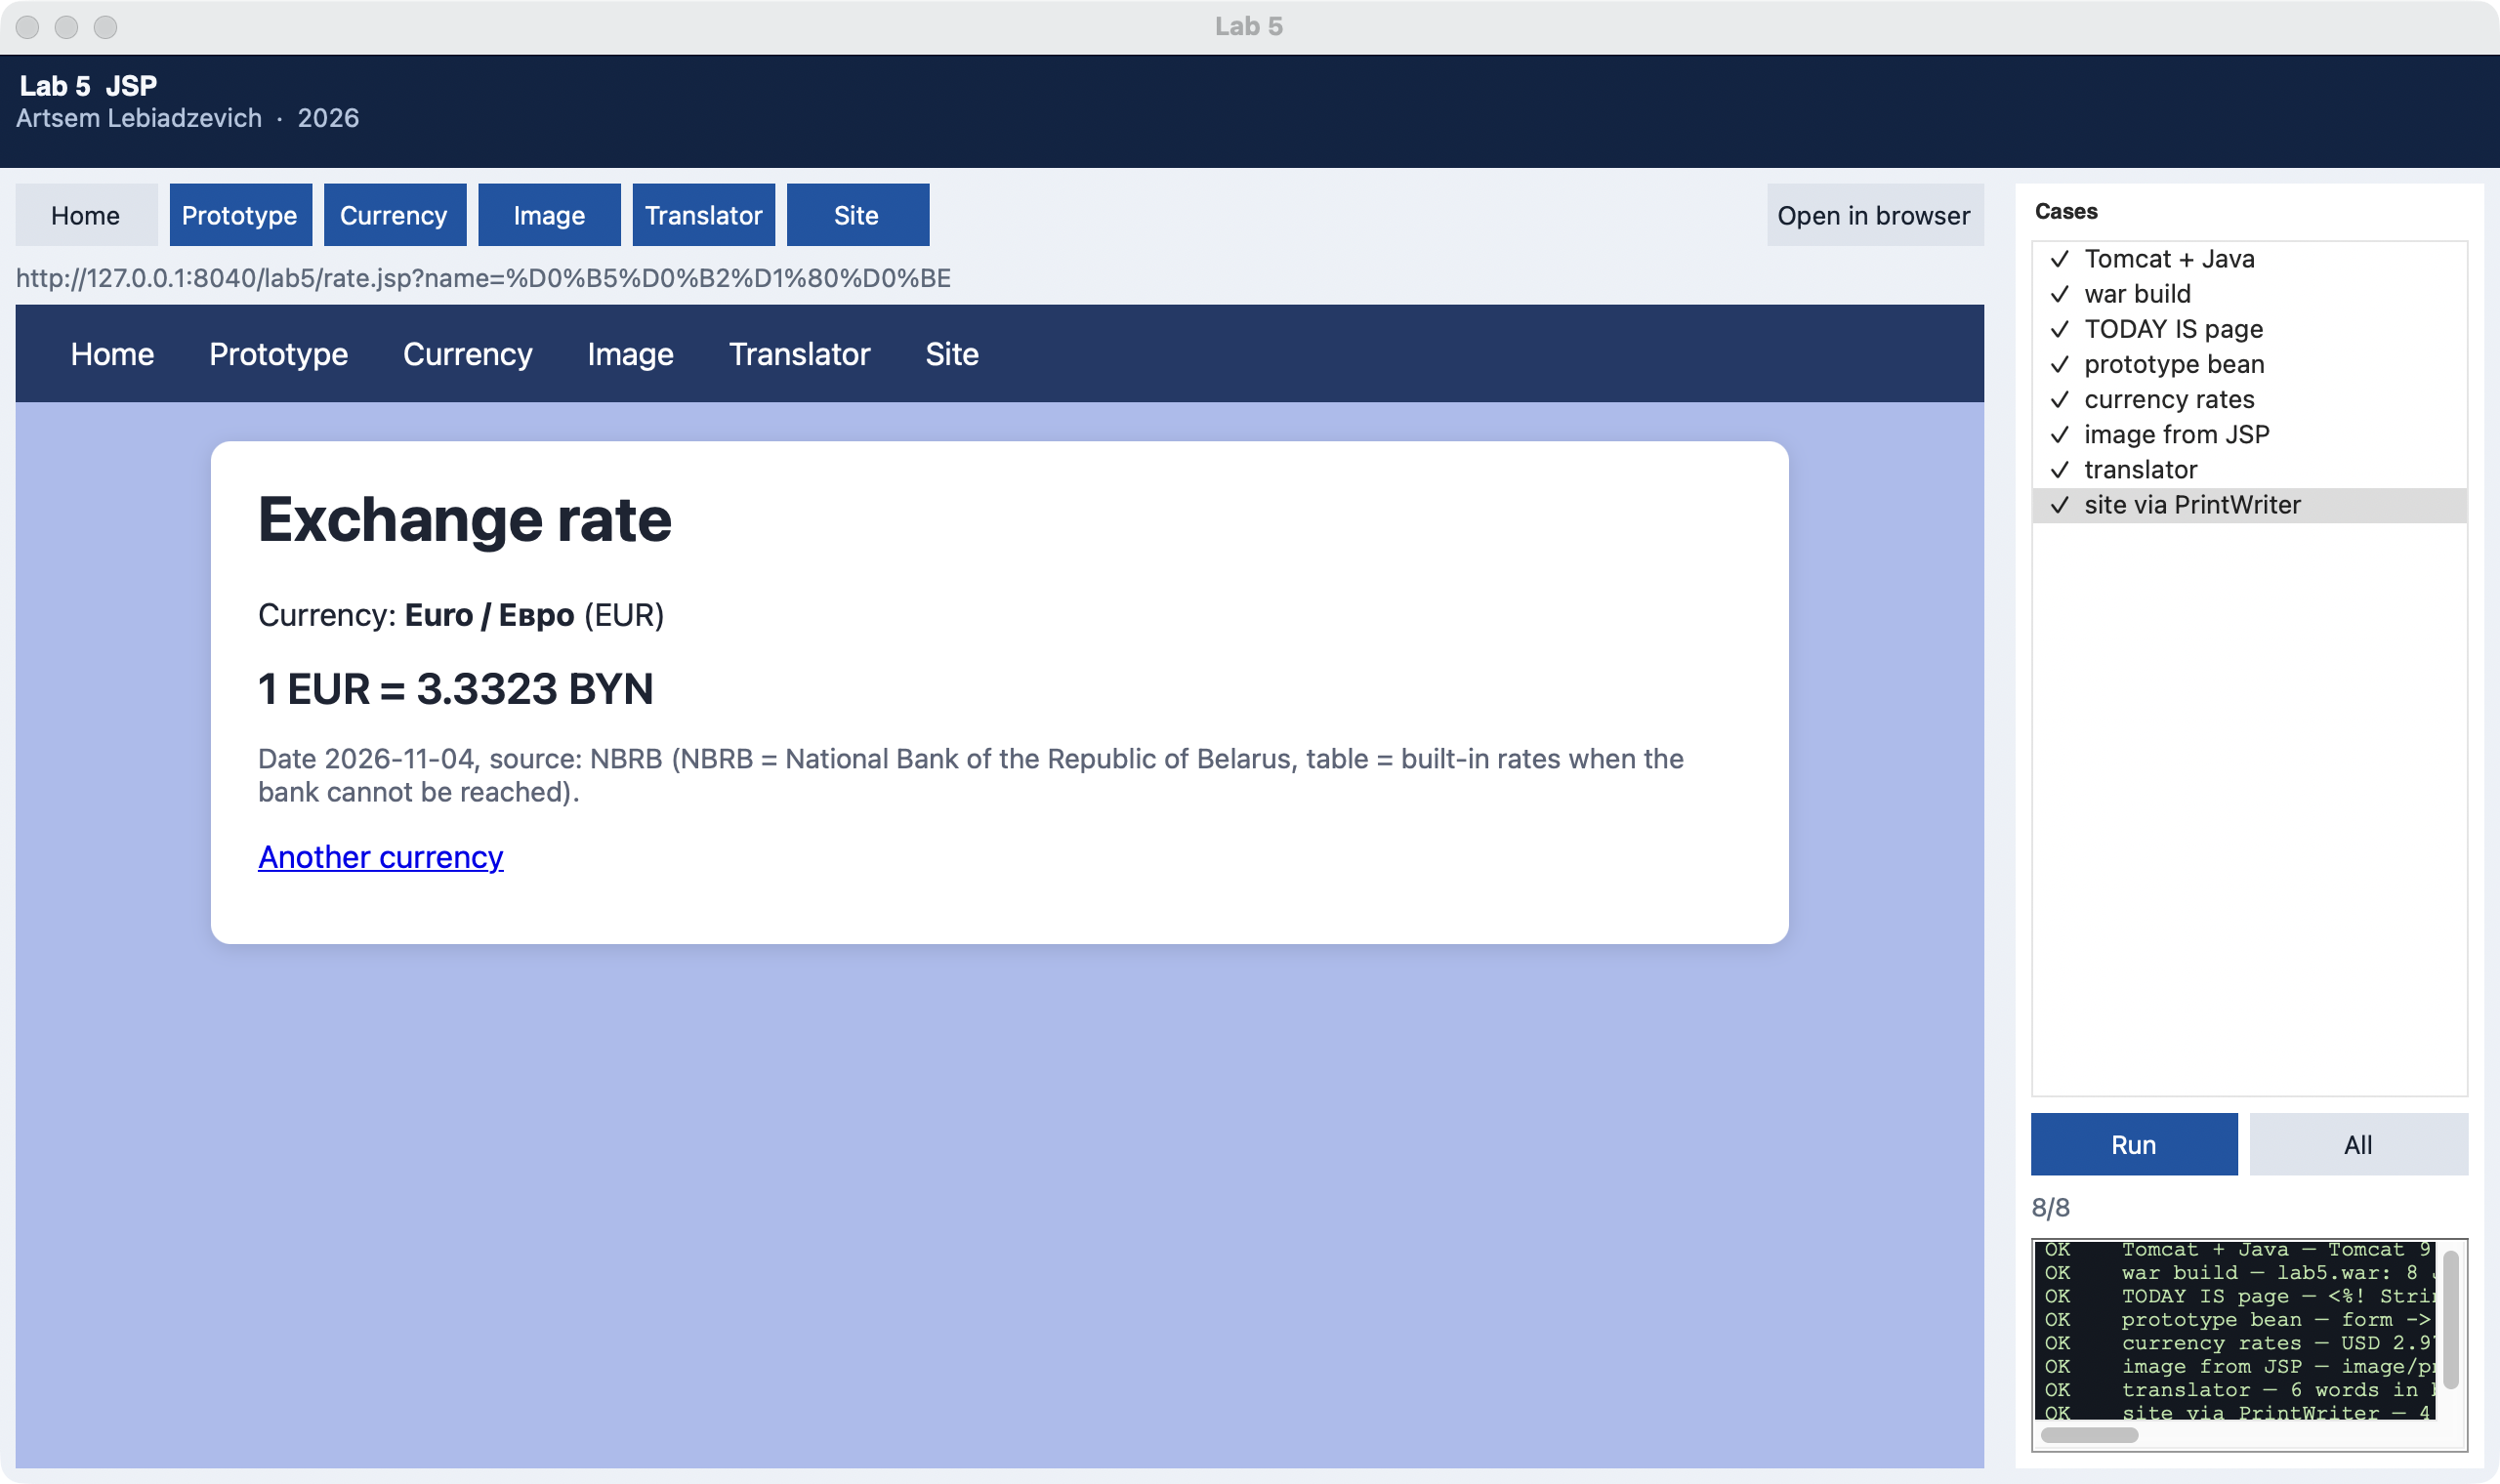
\includegraphics[width=0.95\textwidth]{../screenshots/lab5_currency.png}
\caption{Задание 1: курс евро по запросу <<евро>>}
\label{fig:currency}
\end{figure}

\begin{figure}[H]
\centering
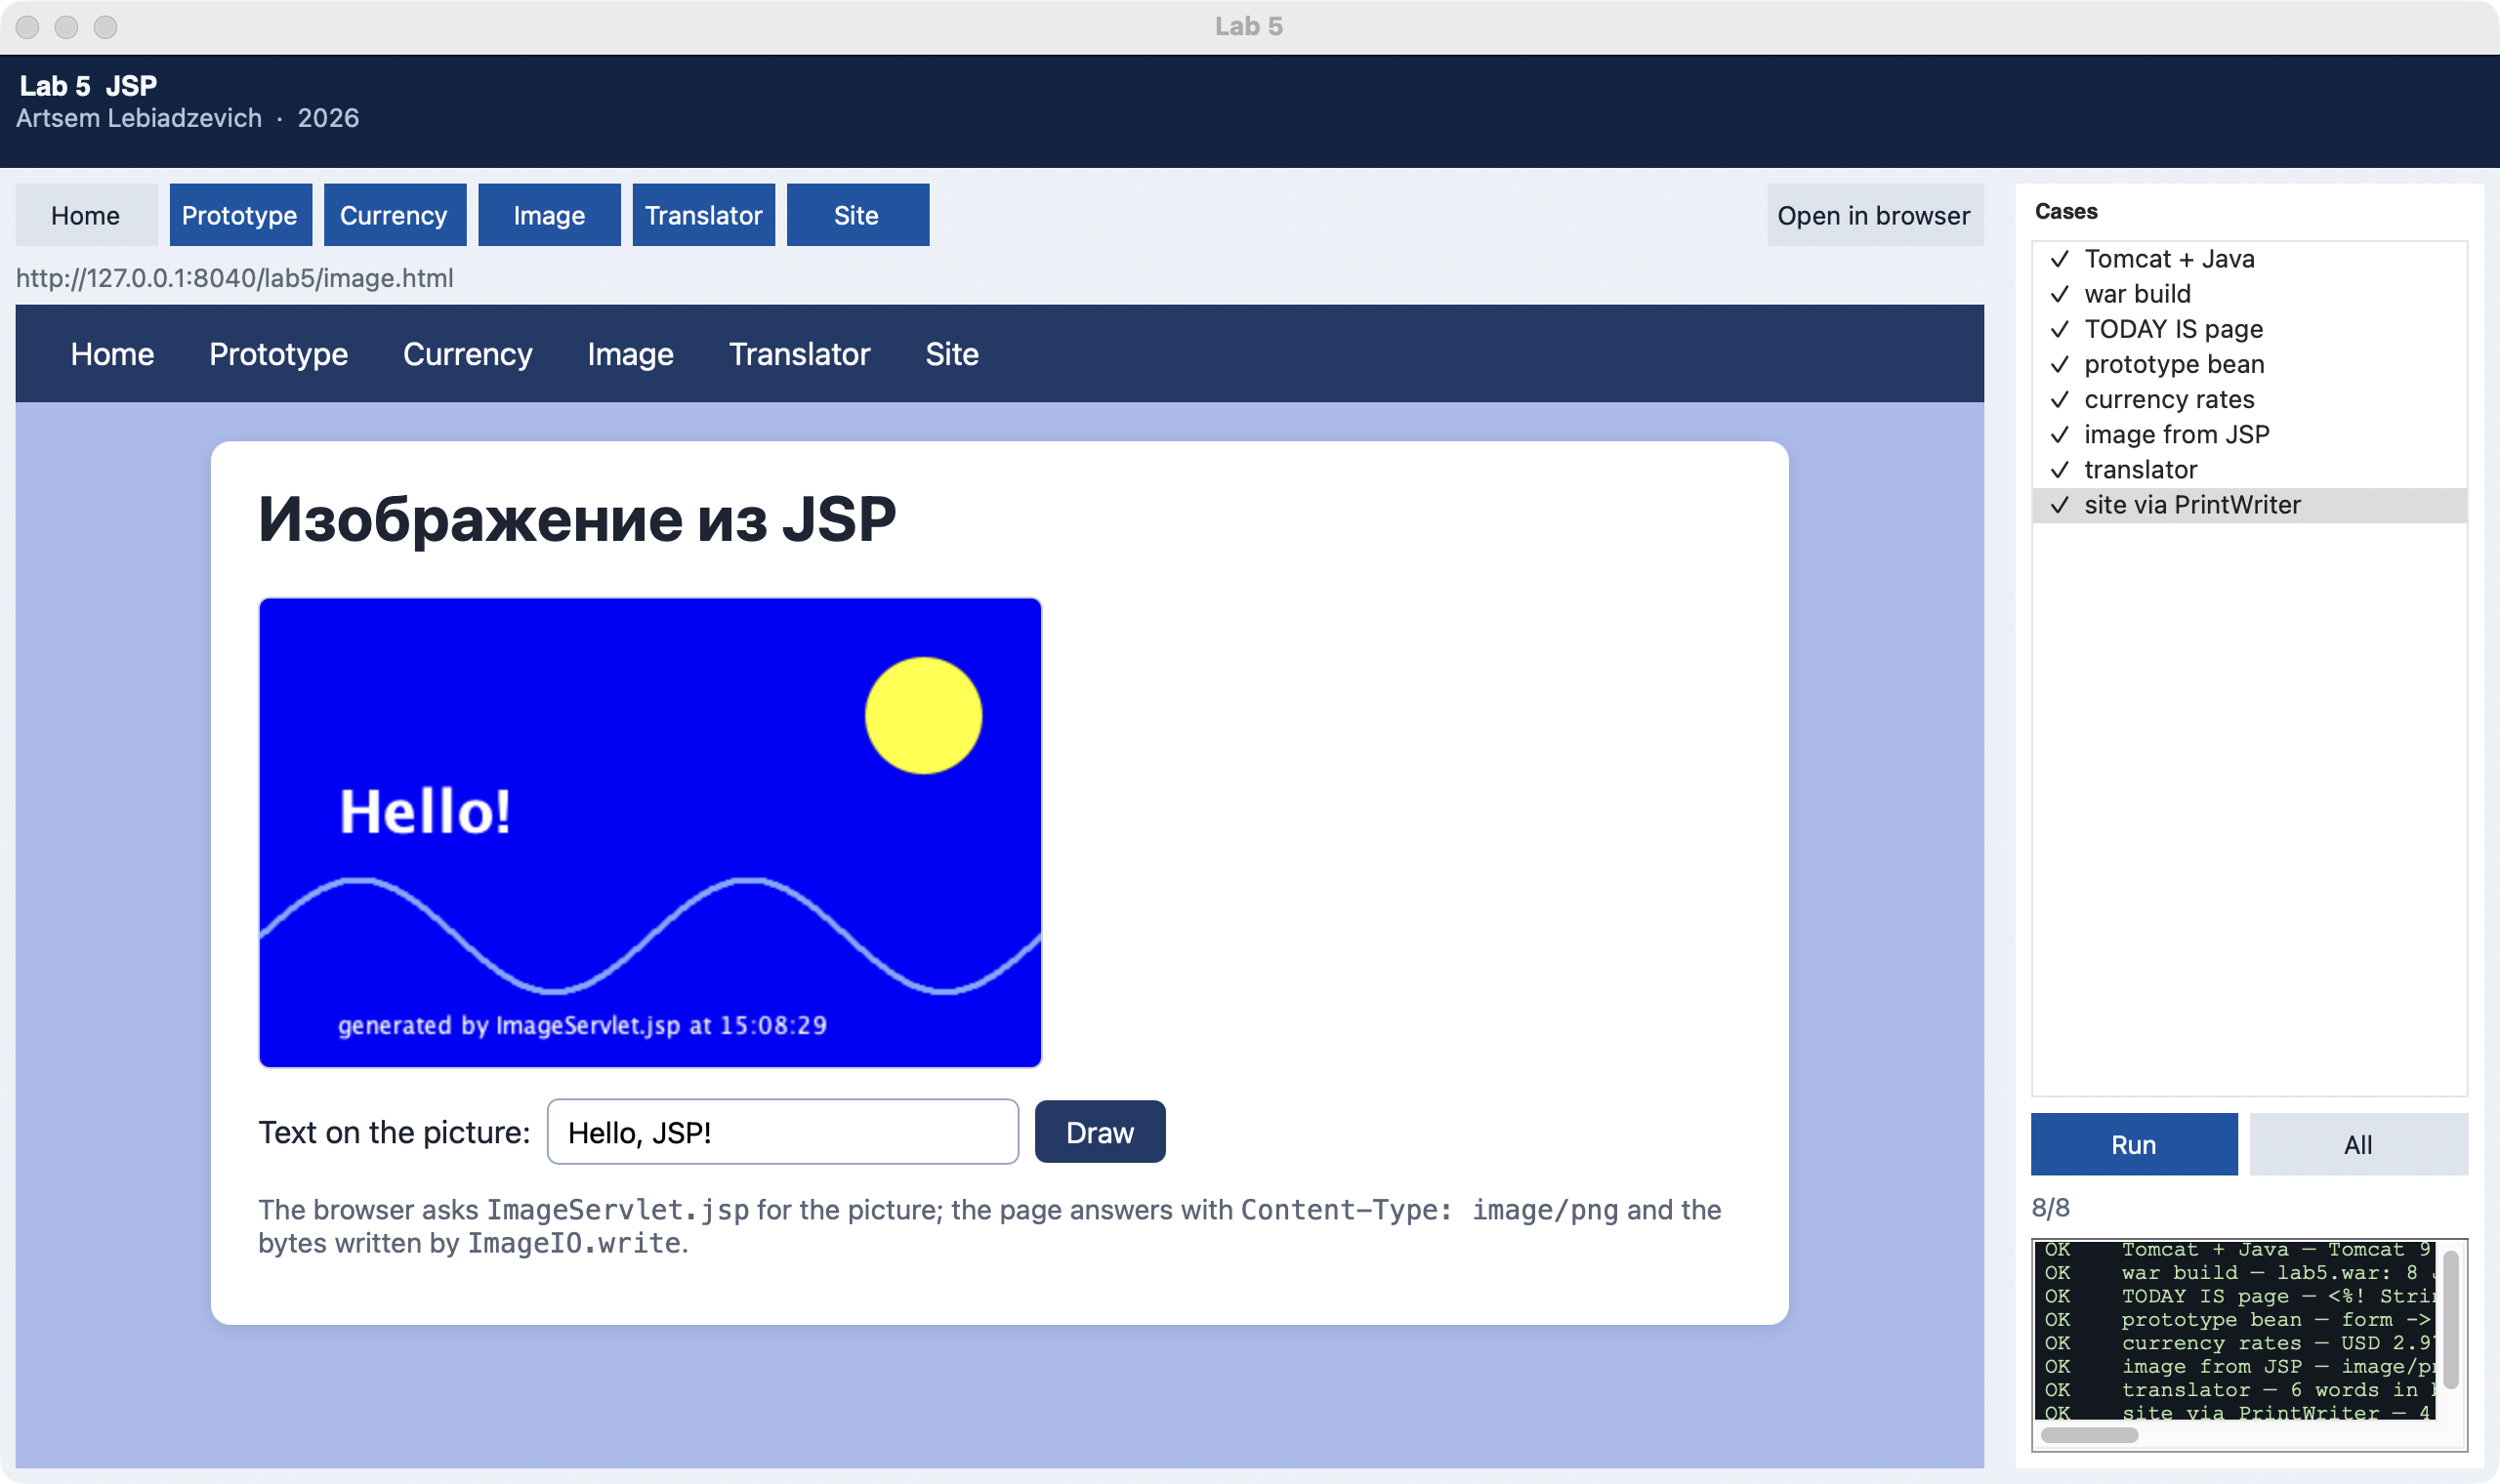
\includegraphics[width=0.95\textwidth]{../screenshots/lab5_image.png}
\caption{Задание 2: изображение, созданное страницей ImageServlet.jsp}
\label{fig:image}
\end{figure}

\begin{figure}[H]
\centering
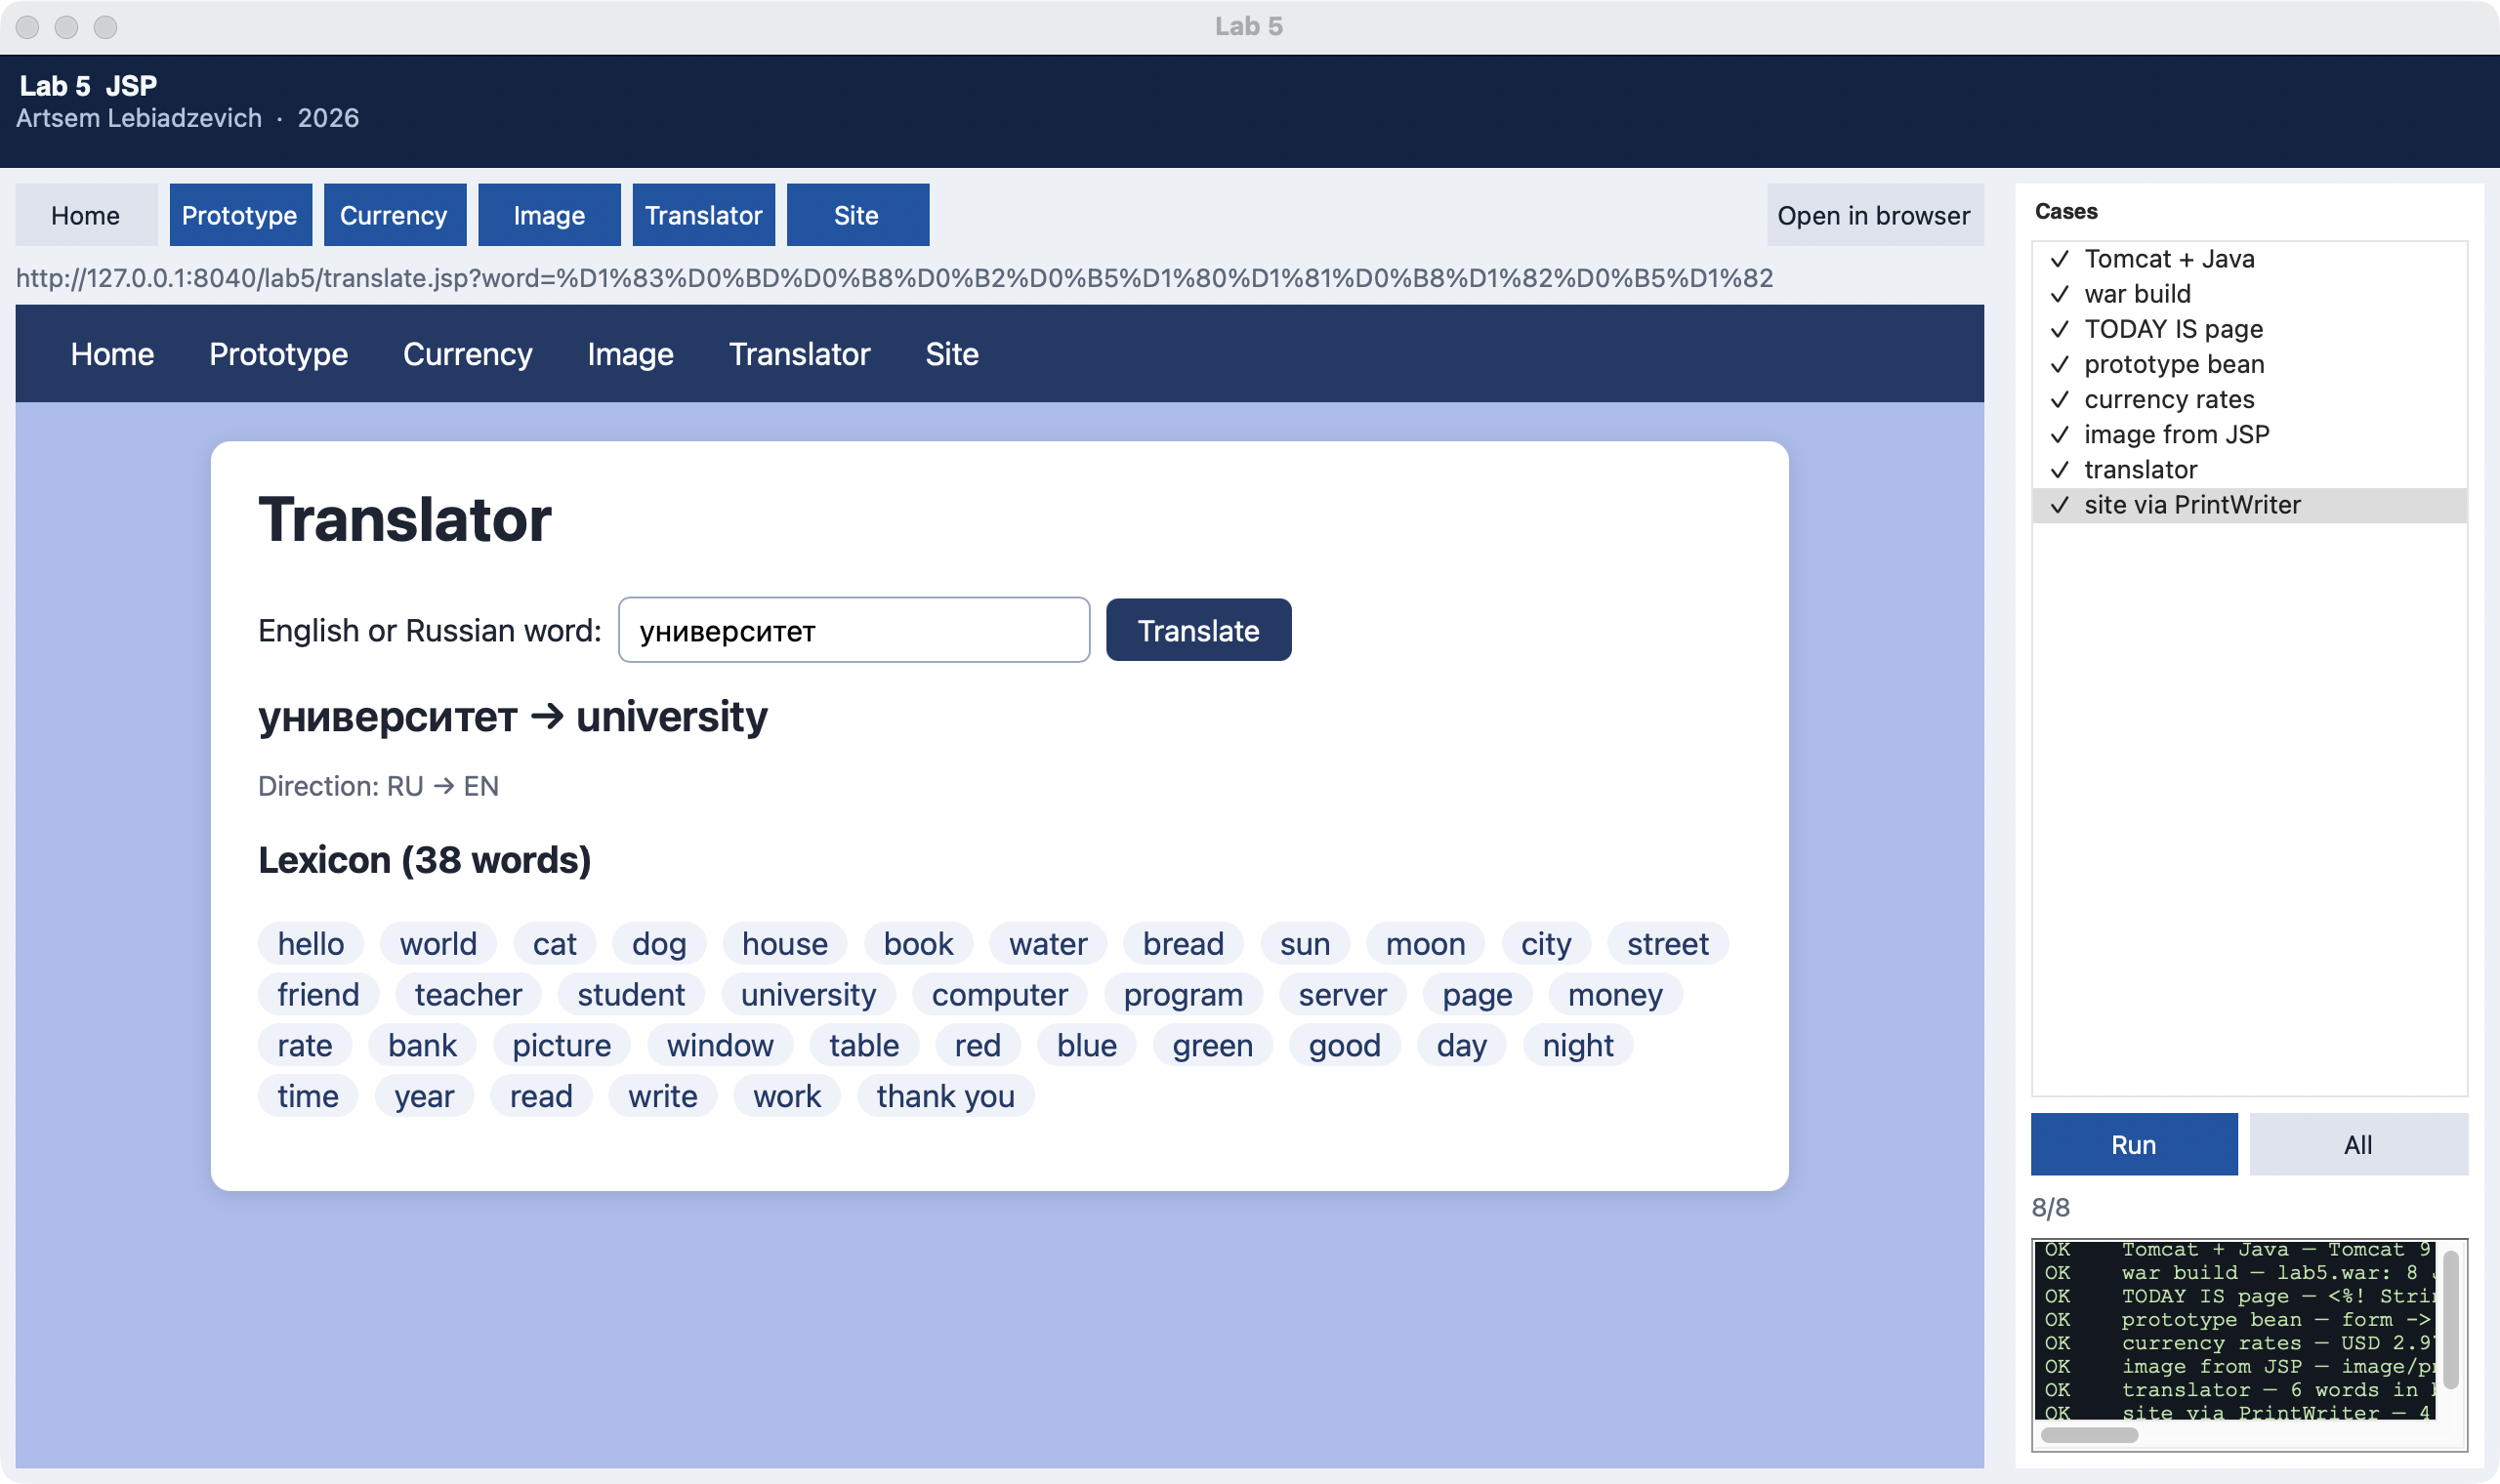
\includegraphics[width=0.95\textwidth]{../screenshots/lab5_translator.png}
\caption{Задание 3: перевод слова <<университет>>}
\label{fig:translator}
\end{figure}

\begin{figure}[H]
\centering
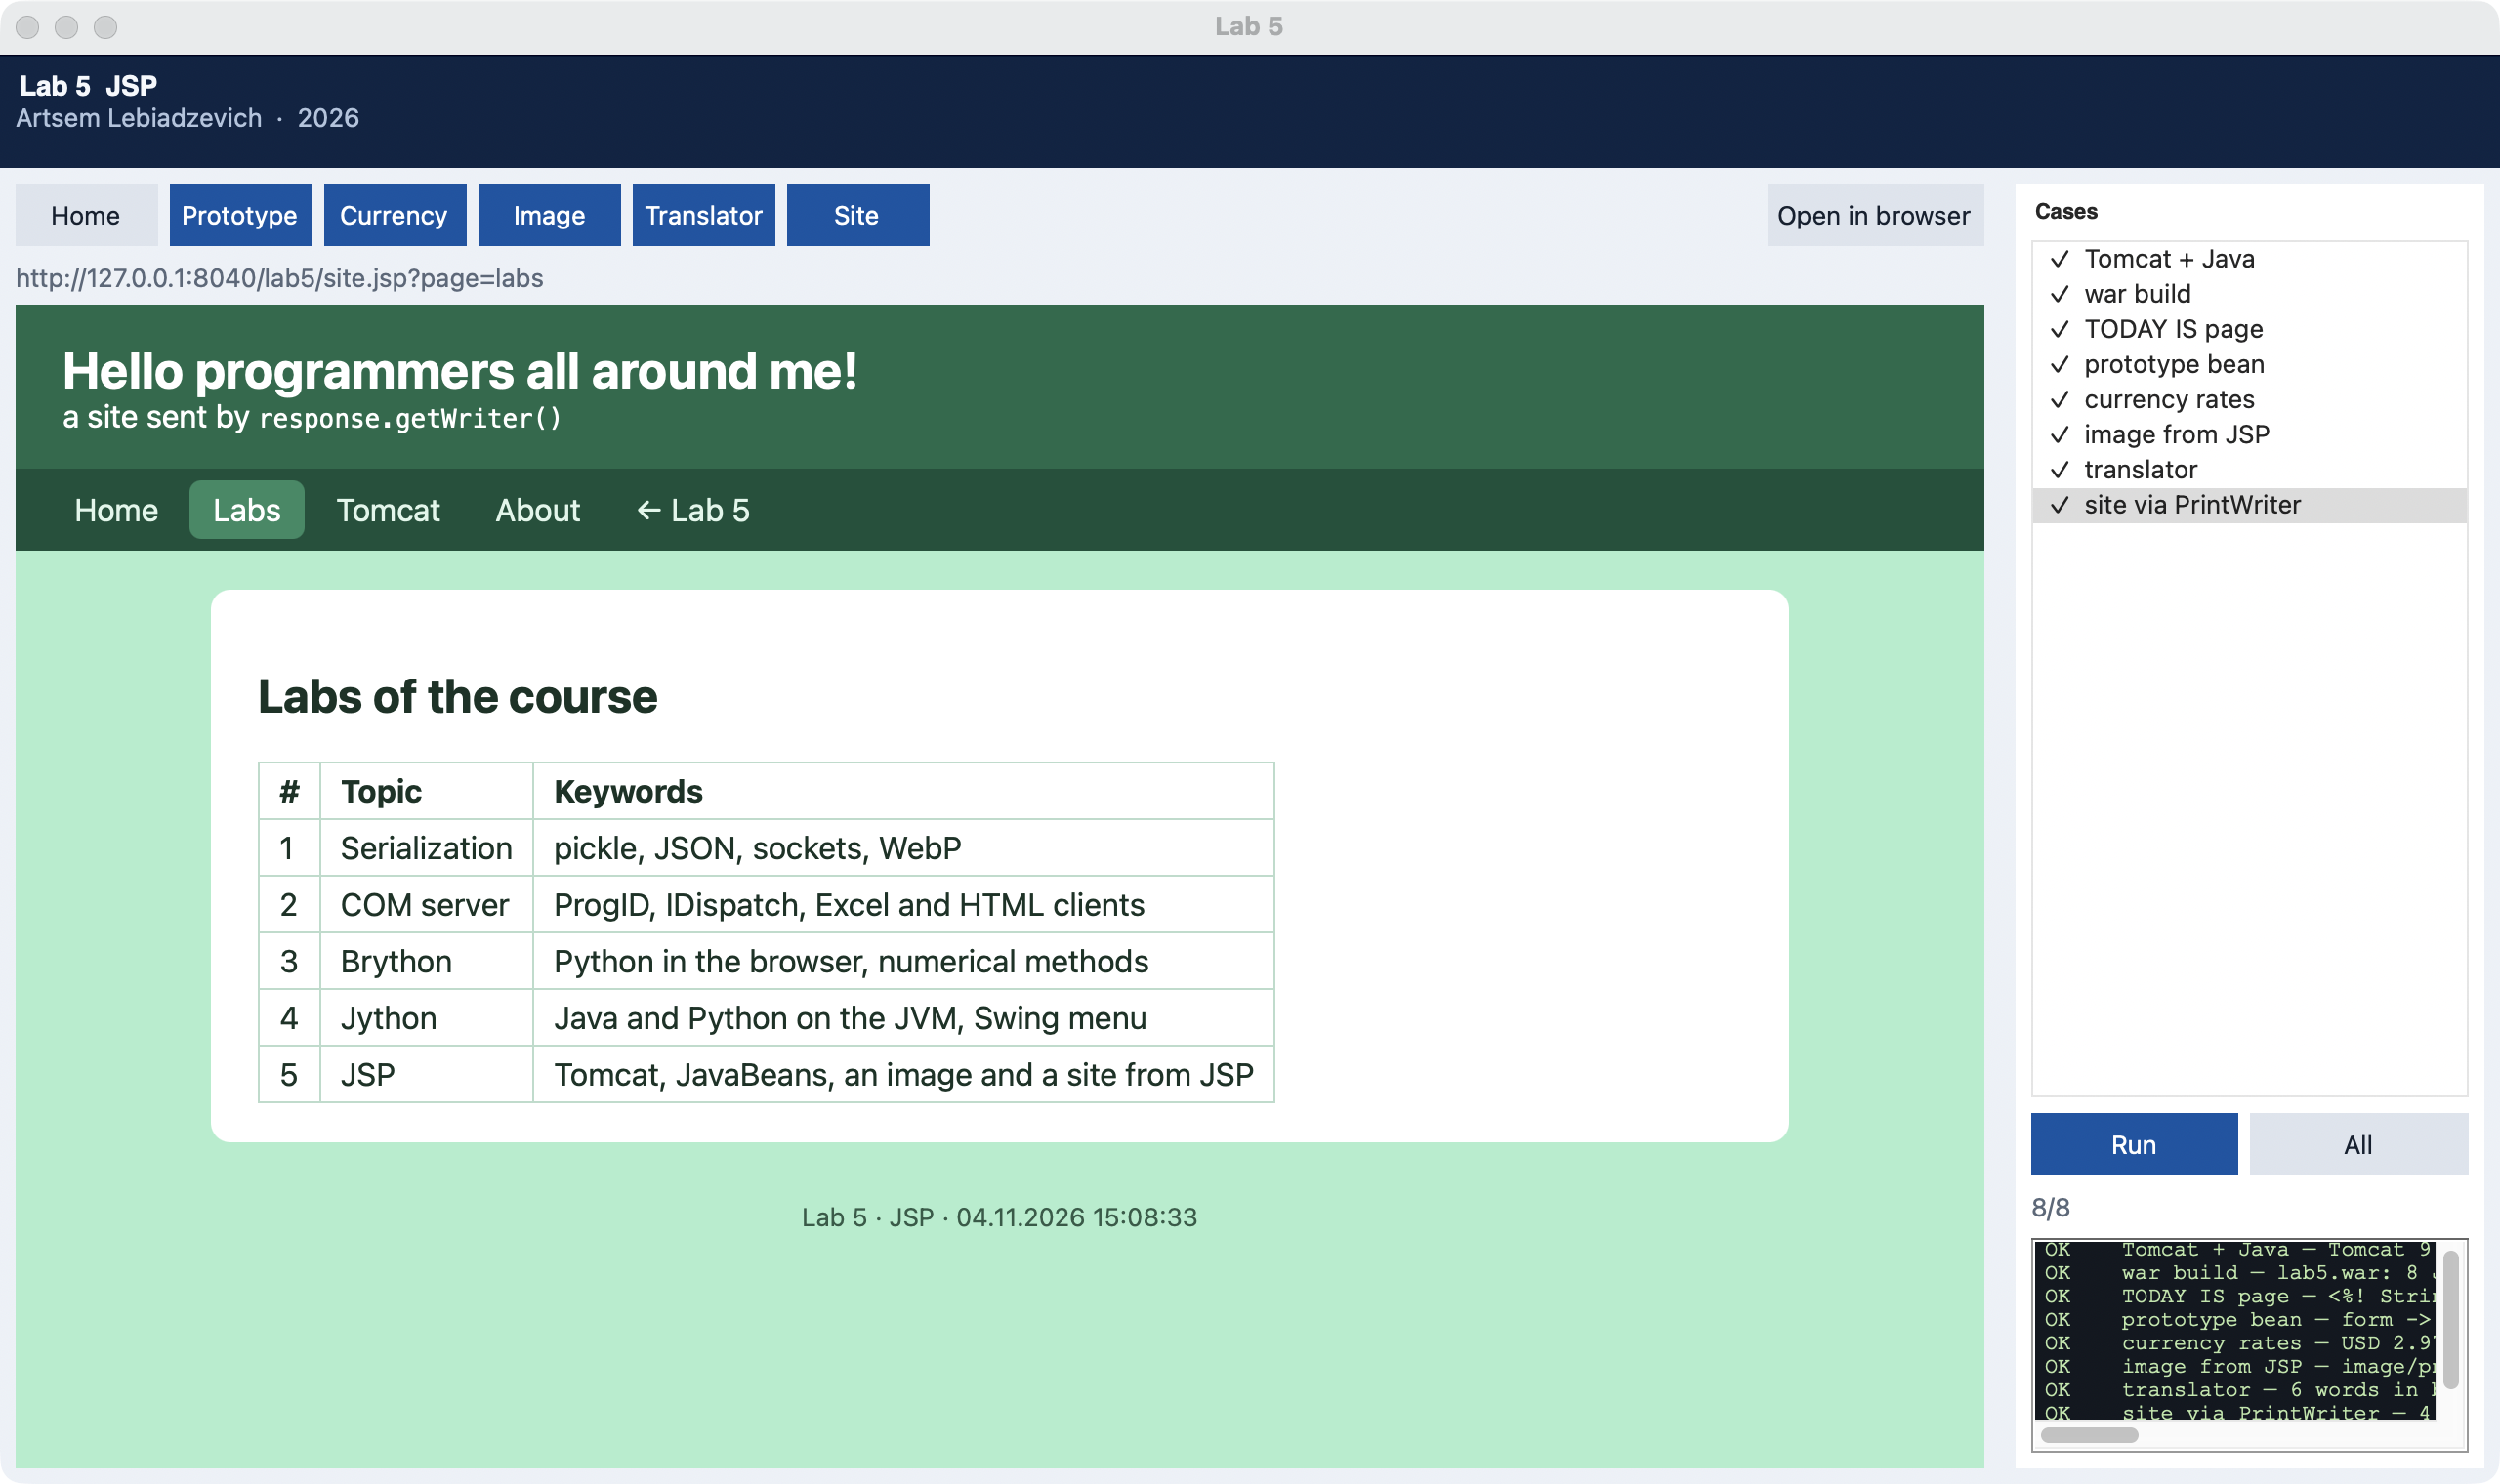
\includegraphics[width=0.95\textwidth]{../screenshots/lab5_site.png}
\caption{Задание 4: сайт, выведенный через PrintWriter}
\label{fig:site}
\end{figure}

Команда \texttt{python main.py -{}-lab 5} собирает архив, запускает Tomcat и выполняет
сценарии без окна; вывод приведён в листинге~\ref{lst:cli}. Что проверяет каждый
сценарий, указано в таблице~\ref{tab:results}.

\lstinputlisting[style=plain, breaklines=true, caption={Вывод программы}, label={lst:cli}]{listings/cli_output.txt}

\begin{table}[H]
\caption{Проверяемые сценарии}
\label{tab:results}
\centering
\small
\begin{tabularx}{\textwidth}{lL}
\toprule
Сценарий & Что проверяется \\
\midrule
environment & версии Tomcat и Java, сервер отвечает \\
war build & в архиве восемь страниц JSP, \texttt{web.xml} и три класса компонентов \\
TODAY IS page & время на странице отличается от времени компьютера не больше чем на
2 минуты \\
prototype bean & \texttt{Hello, Oleg!}; повторный запрос без параметра сохраняет имя в
сессии \\
currency rates & шесть написаний названий дают USD или EUR; курс в разумных пределах,
евро дороже доллара; компонент сессии помнит валюту; <<yen>> отклоняется \\
image from JSP & тип \texttt{image/png}, размер $400\times240$, синий фон, жёлтое солнце
и белые пиксели текста в заданных точках \\
translator & шесть слов в обоих направлениях без учёта регистра и пробелов;
неизвестное слово выводится экранированным \\
site via PrintWriter & четыре страницы, кодировка UTF-8, отмеченный пункт меню;
неизвестная страница заменяется главной \\
\bottomrule
\end{tabularx}
\end{table}

Автоматические тесты (\texttt{python -m unittest tests.test\_labs}) повторяют эти
проверки и пропускаются, если не найдены Java или Tomcat. Все тесты проходят.

\section{Ответы на контрольные вопросы}

\textbf{1. Что такое JSP и как выполняется страница?} HTML-документ со вставками на
Java. При первом обращении Tomcat (Jasper) создаёт из страницы сервлет, компилирует его
и далее вызывает метод \texttt{\_jspService} для каждого запроса.

\textbf{2. Какие теги используются в JSP?} Комментарий \texttt{<\%-{}- -{}-\%>},
директивы \texttt{<\%@ page \%>} и \texttt{<\%@ include \%>}, объявление
\texttt{<\%! \%>}, скриптлет \texttt{<\% \%>}, выражение \texttt{<\%= \%>} и действия
\texttt{jsp:useBean}, \texttt{jsp:setProperty}, \texttt{jsp:getProperty}.

\textbf{3. Что такое JavaBean и как его использует JSP?} Класс с конструктором без
параметров и свойствами \texttt{get}/\texttt{set}. \texttt{jsp:useBean} создаёт или
находит компонент в области видимости, \texttt{jsp:setProperty} заполняет свойство из
одноимённого параметра запроса, \texttt{jsp:getProperty} выводит его значение.

\textbf{4. Как JSP-страница возвращает изображение?} Устанавливает тип
\texttt{image/png}, рисует в \texttt{BufferedImage} и записывает его методом
\texttt{ImageIO.write} в \texttt{response.getOutputStream()}. HTML-страница ссылается на
неё тегом \texttt{<img>}.

\textbf{5. Как разместить web-приложение на Tomcat?} Упаковать его в архив WAR
(\texttt{jar -cvf app.war ...}) с \texttt{WEB-INF/web.xml} и классами в
\texttt{WEB-INF/classes} и скопировать в каталог \texttt{webapps}; Tomcat распакует
архив и опубликует приложение по адресу \texttt{/app/}.

\sectioncenter{Заключение}

В ходе лабораторной работы изучена технология JSP и компоненты JavaBeans на сервере
Tomcat. Выполнены примеры методических материалов и все четыре задания: курсы доллара и
евро по названию валюты (с данными Национального банка), изображение PNG,
сгенерированное JSP-страницей, переводчик из ограниченного лексикона в обе стороны и
сайт, переданный клиенту через \texttt{PrintWriter}.

Практический вывод: JSP-страница компилируется на сервере, поэтому версия Tomcat должна
соответствовать версии Java --- Tomcat 8.5.5 из методички на JDK 17 не компилирует
страницы, обращающиеся к \texttt{System}, и потребовался Tomcat 9. Компоненты выносят
логику из страницы, а область \texttt{session} сохраняет их между запросами. Одна и та
же страница может вернуть HTML, изображение или сайт, сформированный программно.

\sectioncenter{Список использованных источников}

\begin{enumerate}
\item Герман, О.~В. JSP: лабораторная работа по дисциплине <<Технологии компонентного
программирования>> / О.~В.~Герман. --- Минск: БГУИР, 2024.
\item Герман, О.~В. Работа с Web: лекция по дисциплине <<Технологии компонентного
программирования>> / О.~В.~Герман. --- Минск: БГУИР, 2024.
\item Apache Tomcat 9 Documentation [Электронный ресурс]. --- Режим доступа:
\url{https://tomcat.apache.org/tomcat-9.0-doc/}.
\item JavaServer Pages Specification 2.3 [Электронный ресурс]. --- Режим доступа:
\url{https://jcp.org/en/jsr/detail?id=245}.
\item API курсов валют Национального банка Республики Беларусь [Электронный ресурс]. ---
Режим доступа: \url{https://www.nbrb.by/apihelp/exrates}.
\end{enumerate}

\end{document}
